\chapter{Data Analysis and Feature Extraction}

\section{TRT Data}
Before extracting features or training models, I looked at the data collected from the experiment. The data consists of the total reading time (TRT) for each word in the text, which is the sum of the reading times for all fixations on that word. The TRT is calculated by summing the durations of all fixations on a word, which gives an indication of how long the participant spent reading that word.

The TRT data for each participant is stored in a CSV file with columns for the participant ID, the text ID, the word ID, the word itself, the sentence ID, the sentence itself, the word index in the sentence, and the TRT for that word. The TRT is measured in milliseconds. 

The figure \ref{fig:trt_data} shows a histogram of the TRT data, which gives an overview of the distribution of reading times across the dataset. As is visible in the histogram, a lot of words have a total reading time of 0 milliseconds, which means that the participant did not fixate on those words at all. This is expected, as some words in the text may be skipped or read very quickly without any fixations. The histogram also shows that there are some words with very high TRT values, which indicates that those words were read more carefully or were more difficult to process.

\begin{figure}
    \centering
    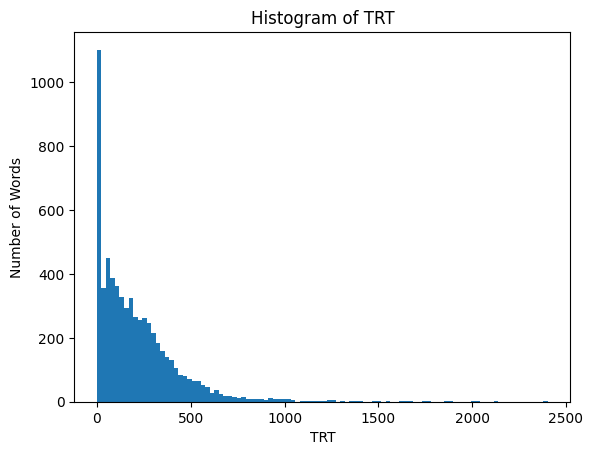
\includegraphics[width=0.8\textwidth]{images/TRT_histogram.png}
    \caption{Histogram of Total Reading Time}
    \label{fig:trt_data}
\end{figure}

\section{Features}
The next step is to extract features from the text that can be used to predict the TRT for each word. I extracted both simple and more complex features. The word features are as follows:

\begin{enumerate}
    \item \textbf{Length:} The number of characters in the word. This feature is simple but effective, as longer words tend to take more time to read.
    
    \item \textbf{Number of tokens:} The number of tokens the word is tokenized into. This feature is useful because the more tokens the word is split into, the longer and more complex it is.
    
    \item \textbf{Frequency:} The frequency of the word in the text. This feature is useful because more frequent words tend to be easier to read and process.
    
    \item \textbf{Surprisal:} The surprisal of the word in the context of the sentence. Surprisal is a measure of how unexpected a word is in a given context, and it is calculated using a language model. I used a pre-trained AutoModelForMaskedLM, \textit{dumitrescustefan/bert-base-romanian-cased-v1}, to calculate the surprisal of each word in the sentence. The surprisal is calculated as the negative logarithm of the probability of the word given the context, which is the sentence in which the word appears. The lower the surprisal, the more predictable the word is in that context.
    
    \item \textbf{Transformer embeddings:} The contextual embedding of the word in the sentence, obtained using a pre-trained transformer model. I used a pre-trained BERT model, \textit{dumitrescustefan/bert-base-romanian-cased-v1}, to obtain the contextual embeddings of each word in the sentence. To make this process more efficient, I first computed the embeddings for each sentence by feeding them through the BERT model and extracting the hidden states from various layers (first, middle, last, and the average across all layers).

    After obtaining the token-level embeddings, I mapped them back to words. Since some words are split into multiple subword tokens by the tokenizer, I averaged the embeddings of all the tokens corresponding to a single word. This mapping was based on character-level offset information provided by the tokenizer. Subword tokens that belong to the same word have contiguous or overlapping character offsets, whereas tokens belonging to different words have non-overlapping offsets. Using this strategy, I reconstructed word-level embeddings from the token embeddings. In the end, I obtained four embeddings for each word: one from the first layer, one from the middle layer, one from the last layer, and one averaged across all layers.
\end{enumerate}

After computing the features for each word, I calculated the Pearson correlation between the features and the total reading time. The results are shown in Table \ref{tab:feature_correlation}. As expected, the length of the word has the highest positive correlation with the TRT, followed by the surprisal and the number of tokens, while the frequency has a similar negative correlation with the TRT. The Pearson correlation is a measure of the linear relationship between two variables, and it ranges from -1 to 1, where -1 indicates a perfect negative correlation, 0 indicates no correlation, and 1 indicates a perfect positive correlation. It is calculated as the covariance of the two variables divided by the product of their standard deviations by the formula:
\begin{equation}
    r = \frac{\text{cov}(X, Y)}{\sigma_X \sigma_Y}
\end{equation}
where \( r \) is the Pearson correlation coefficient, \( X \) and \( Y \) are the two variables, \( \text{cov}(X, Y) \) is the covariance between \( X \) and \( Y \), and \( \sigma_X \) and \( \sigma_Y \) are the standard deviations of \( X \) and \( Y \), respectively.

\begin{table}
    \centering
    \begin{tabular}{|l|c|}
        \hline
        Feature & Correlation with TRT \\
        \hline
        Length & 0.59 \\
        Number of tokens & 0.30 \\
        Frequency & -0.35 \\
        Surprisal & 0.34 \\
        \hline
    \end{tabular}
    \caption{Correlation between features and total reading time (TRT).}
    \label{tab:feature_correlation}
\end{table}